\documentclass[dvipdfmx]{jarticle}
\usepackage{graphicx}
\usepackage{here}
\usepackage{ascmac}
\usepackage{amsmath,amssymb}
\usepackage[margin=20mm]{geometry}
\usepackage{listings,jvlisting} %日本語のコメントアウトをする場合jvlisting(もしくはjlisting)が必要
%ここからソースコードの表示に関する設定
\lstset{
  basicstyle={\ttfamily},
  identifierstyle={\small},
  commentstyle={\smallitshape},
  keywordstyle={\small\bfseries},
  ndkeywordstyle={\small},
  stringstyle={\small\ttfamily},
  frame={tb},
  breaklines=true,
  columns=[l]{fullflexible},
  numbers=left,
  xrightmargin=0zw,
  xleftmargin=3zw,
  numberstyle={\scriptsize},
  stepnumber=1,
  numbersep=1zw,
  lineskip=-0.5ex
}
\setcounter{tocdepth}{4}
\pagestyle{empty}
\begin{document}
\title{計算機科学実験及演習4 データベース 最終課題}S
\author{1029-32-6611 山田裕晃}
\maketitle

\section{システム概要}

このアプリケーションは「各種イベントの登録・予約を行い、当日の受付をQRコードによるチケット読み取りによって行うアプリケーション」である。

昨今の新型コロナウイルスの流行により、ライブに限らず、規模を問わず様々なイベントにおいて予約による人数制限を設けるような事例も多く見られるようになった。
これらの需要に応えるため、「シンプルかつ使いやすい予約アプリケーション」をコンセプトに設計を行うことにした。

\subsection{利用者の役割の列挙と説明}
以下に挙げる役割を想定している。
\subsubsection{参加者}
イベントに参加する者。各種イベントに申し込み、チケットを発券し、当日受付を済ませることでイベントに参加できる。
\subsubsection{主催者}
イベントの主催者。各種イベントをアプリケーション上に登録し、定員などのイベント情報を管理できる。
\subsubsection{スタッフ}
イベント当日のスタッフ。イベント当日に参加者に提示されたチケットを読み取って受付を行うことができる。

\subsection{役割ごとの機能の列挙と説明}
以下に挙げる機能を想定している。
\subsubsection{ログイン-共通}
IDとパスワードを入力することでログインできる。
\subsubsection{イベント一覧の確認-参加者}
アプリケーション上に登録されているイベント一覧を表示する。
\subsubsection{イベントへの予約-参加者}
参加したいイベントを選択し、定員に空きがあれば申し込むことができる。
\subsubsection{チケットの表示-参加者}
申し込みをしたチケット一覧、及びそれぞれのチケットを表示する。
それぞれのチケットにはQRコードが記載されており、当日これをスマホ等でスタッフに表示することで受付できる。
\subsubsection{イベントの登録-主催者}
新たにイベントを開催したい場合、イベントを登録できる。
\subsubsection{イベント情報の設定-主催者}
イベントの開催場所・定員などの情報を編集できる。
\subsubsection{予約状況の確認-主催者}
定員に対する予約状況などを確認できる。
\subsubsection{チケットの受付-スタッフ}
参加者が提示したチケットに表示されたQRコードを読み込むことで受付できる。


\section{実体関連図}

\begin{figure}[H]
  \centering
  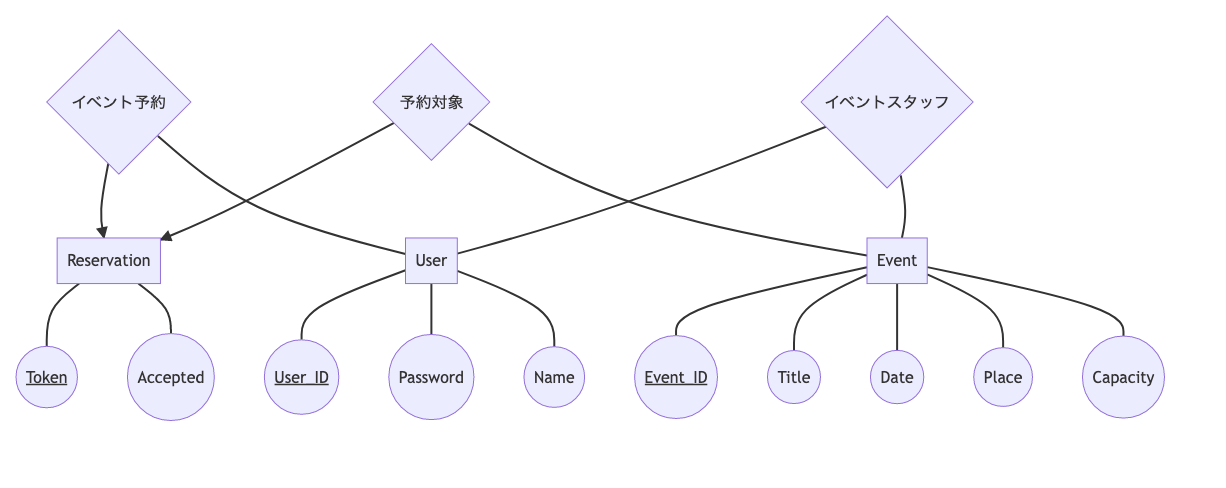
\includegraphics[scale=0.4]{ermodel.png}
  \caption{実体関連図}
\end{figure}

\subsection{ユーザー(User)}
参加者・主催者・スタッフに共通の実体集合。
ID・パスワード(password)・名前(name)を属性として持つ。

\subsection{イベント(Event)}
イベントを表現する実体集合。
ID・イベント名(title)・開催日時(date)・開催場所(place)・定員(capacity)を属性として持つ。

\subsection{予約(Reservation)}
1件の予約を表す実体集合。あるユーザーが、あるイベントに申し込んだ際に生成される。
トークン(token)と受付状態(accepted)を属性として持つ。
トークンはユニークに生成される文字列であり、主キー及びQRコードの発行のために利用される。

\subsection{各関連集合}
ユーザーと予約の間には、「ユーザーが予約を行う」という関係が存在する。
ユーザーは予約を複数件行うことができるため、ユーザーと予約は一対多の関係である。

また、予約とイベントの間には、「あるイベントに対して予約がなされる」という関係が存在する。
イベントには複数件の予約がなされるため、イベントと予約は一対多の関係である。

ユーザーとイベントの間には、「あるイベントの主催者/スタッフである」という関係が存在する。
イベントの主催者/スタッフは複数になりうる。
また、あるイベントのスタッフであるユーザーが他のイベントでもスタッフを務めるという可能性もありうるので、
ユーザーとイベントは多対多の関係である。


\section{関係スキーマ}

\begin{table}[H]
  \centering
   \begin{tabular}{|r|l|l|}
    \hline
    ユーザーID & 名前 & パスワード \\
    \hline \hline
    1 & 山田 & yamada \\
    2 & 伊藤 & ito \\
    3 & 下田 & shimoda \\
    4 & 加藤 & kato \\
    \hline
  \end{tabular}
  \caption{ユーザー}
\end{table}

\begin{table}[H]
  \centering
   \begin{tabular}{|r|l|r|l|r|}
    \hline
    イベントID & イベント名 & 日時 & 場所 & 定員 \\
    \hline \hline
    1 & 京都大学11月祭 & 2022/11/19 & 京都大学 & 1000 \\
    2 & 計算機科学実験及演習4 & 2022/10/20 & 総合研究7号館 & 40 \\
    \hline
  \end{tabular}
  \caption{イベント}
\end{table}

\begin{table}[H]
  \centering
   \begin{tabular}{|r|r|l|r|}
    \hline
    ユーザーID & イベントID & トークン & 受付状態 \\
    \hline \hline
    1 & 1 & abcde & 0 \\
    1 & 2 & fghij & 1 \\
    2 & 2 & klmno & 1 \\
    3 & 1 & pqrst & 0 \\
    4 & 2 & uvwxy & 0 \\
    \hline
  \end{tabular}
  \caption{予約}
\end{table}


\section{機能・インタフェース}

\section{工夫点}

\section{感想}

\section{課題1〜3からの変更事項}
課題3で設計していた関係スキーマでは、関係「イベントスタッフ」が表現できていなかったため、
新たに「スタッフ」を追加することにした。

また、主催者はスタッフの一部とみなし、関係「イベントスタッフ」に「スタッフ権限」という名前の属性を追加することで
主催者か否かの判別をする仕様に変更した。

「スタッフ」は、属性にユーザーIDとイベントIDとスタッフ権限を持ち、主キーは「ユーザーID」と「イベントID」の複合主キーである。

それに伴い、以下の関数従属性が追加される。
\begin{itemize}
  \item {ユーザーID, イベントID} $\rightarrow$ {スタッフ権限}
\end{itemize}

新たに正規化しなおした関係スキーマを提示する。
\begin{description}
  \item[ユーザー] \underline{ユーザーID}, 名前, パスワード
  \item[イベント] \underline{イベントID}, イベント名, 開催日時, 開催場所, 定員
  \item[予約] ユーザーID, イベントID, \underline{トークン}, 受付状態
  \item[スタッフ] \underline{ユーザーID}, \underline{イベントID}, スタッフ権限
\end{description}

\end{document}